\begin{tikzpicture}
  \node (cleanImage) at (0, 0) {
    \includegraphics[width = 1.4cm]{images/dog_clean.jpg}
  };

  \node (perturbedImage) at (2.5, -2) {
    \includegraphics[width = 1.4cm]{images/dog_perturbation.jpg}
  };

  \node (teacher) at (5, 2) {
    \scalebox{0.15}{
      \begin{tikzpicture}[xscale = 3]
  \node[draw, circle] (N11) at (0, 0){
  };

  \node[draw, circle] (N21) at (0, -1){
  };

  \node[draw, circle] (N31) at (0, -2){
  };

  \node[draw, circle] (N41) at (0, -3){
  };

  \node[draw, circle] (N51) at (0, -4){
  };

  \node[draw, circle] (N61) at (0, -5){
  };

  \node[draw, circle] (N71) at (0, -6){
  };

  \node[draw, circle] (N81) at (0, -7){
  };

  \node[draw, circle] (N91) at (0, -8){
  };

  \node[draw, circle] (N12) at (1, 0){
  };

  \node[draw, circle] (N22) at (1, -1){
  };

  \node[draw, circle] (N32) at (1, -2){
  };

  \node[draw, circle] (N42) at (1, -3){
  };

  \node[draw, circle] (N52) at (1, -4){
  };

  \node[draw, circle] (N62) at (1, -5){
  };

  \node[draw, circle] (N72) at (1, -6){
  };

  \node[draw, circle] (N82) at (1, -7){
  };

  \node[draw, circle] (N92) at (1, -8){
  };

  \node[draw, circle] (N13) at (2, 0){
  };

  \node[draw, circle] (N23) at (2, -1){
  };

  \node[draw, circle] (N33) at (2, -2){
  };

  \node[draw, circle] (N43) at (2, -3){
  };

  \node[draw, circle] (N53) at (2, -4){
  };

  \node[draw, circle] (N63) at (2, -5){
  };

  \node[draw, circle] (N73) at (2, -6){
  };

  \node[draw, circle] (N83) at (2, -7){
  };

  \node[draw, circle] (N93) at (2, -8){
  };

  \node[draw, circle] (N14) at (3, -3.5){
  };

  \node[draw, circle] (N24) at (3, -4.5){
  };

  \draw[->] (N11) -- (N12);
  \draw[->] (N11) -- (N22);
  \draw[->] (N11) -- (N32);
  \draw[->] (N11) -- (N42);
  \draw[->] (N11) -- (N52);
  \draw[->] (N11) -- (N62);
  \draw[->] (N11) -- (N72);
  \draw[->] (N11) -- (N82);
  \draw[->] (N11) -- (N92);
  \draw[->] (N21) -- (N12);
  \draw[->] (N21) -- (N22);
  \draw[->] (N21) -- (N32);
  \draw[->] (N21) -- (N42);
  \draw[->] (N21) -- (N52);
  \draw[->] (N21) -- (N62);
  \draw[->] (N21) -- (N72);
  \draw[->] (N21) -- (N82);
  \draw[->] (N21) -- (N92);
  \draw[->] (N31) -- (N12);
  \draw[->] (N31) -- (N22);
  \draw[->] (N31) -- (N32);
  \draw[->] (N31) -- (N42);
  \draw[->] (N31) -- (N52);
  \draw[->] (N31) -- (N62);
  \draw[->] (N31) -- (N72);
  \draw[->] (N31) -- (N82);
  \draw[->] (N31) -- (N92);
  \draw[->] (N41) -- (N12);
  \draw[->] (N41) -- (N22);
  \draw[->] (N41) -- (N32);
  \draw[->] (N41) -- (N42);
  \draw[->] (N41) -- (N52);
  \draw[->] (N41) -- (N62);
  \draw[->] (N41) -- (N72);
  \draw[->] (N41) -- (N82);
  \draw[->] (N41) -- (N92);
  \draw[->] (N51) -- (N12);
  \draw[->] (N51) -- (N22);
  \draw[->] (N51) -- (N32);
  \draw[->] (N51) -- (N42);
  \draw[->] (N51) -- (N52);
  \draw[->] (N51) -- (N62);
  \draw[->] (N51) -- (N72);
  \draw[->] (N51) -- (N82);
  \draw[->] (N51) -- (N92);
  \draw[->] (N61) -- (N12);
  \draw[->] (N61) -- (N22);
  \draw[->] (N61) -- (N32);
  \draw[->] (N61) -- (N42);
  \draw[->] (N61) -- (N52);
  \draw[->] (N61) -- (N62);
  \draw[->] (N61) -- (N72);
  \draw[->] (N61) -- (N82);
  \draw[->] (N61) -- (N92);
  \draw[->] (N71) -- (N12);
  \draw[->] (N71) -- (N22);
  \draw[->] (N71) -- (N32);
  \draw[->] (N71) -- (N42);
  \draw[->] (N71) -- (N52);
  \draw[->] (N71) -- (N62);
  \draw[->] (N71) -- (N72);
  \draw[->] (N71) -- (N82);
  \draw[->] (N71) -- (N92);
  \draw[->] (N81) -- (N12);
  \draw[->] (N81) -- (N22);
  \draw[->] (N81) -- (N32);
  \draw[->] (N81) -- (N42);
  \draw[->] (N81) -- (N52);
  \draw[->] (N81) -- (N62);
  \draw[->] (N81) -- (N72);
  \draw[->] (N81) -- (N82);
  \draw[->] (N81) -- (N92);
  \draw[->] (N91) -- (N12);
  \draw[->] (N91) -- (N22);
  \draw[->] (N91) -- (N32);
  \draw[->] (N91) -- (N42);
  \draw[->] (N91) -- (N52);
  \draw[->] (N91) -- (N62);
  \draw[->] (N91) -- (N72);
  \draw[->] (N91) -- (N82);
  \draw[->] (N91) -- (N92);
  \draw[->] (N12) -- (N13);
  \draw[->] (N12) -- (N23);
  \draw[->] (N12) -- (N33);
  \draw[->] (N12) -- (N43);
  \draw[->] (N12) -- (N53);
  \draw[->] (N12) -- (N63);
  \draw[->] (N12) -- (N73);
  \draw[->] (N12) -- (N83);
  \draw[->] (N12) -- (N93);
  \draw[->] (N22) -- (N13);
  \draw[->] (N22) -- (N23);
  \draw[->] (N22) -- (N33);
  \draw[->] (N22) -- (N43);
  \draw[->] (N22) -- (N53);
  \draw[->] (N22) -- (N63);
  \draw[->] (N22) -- (N73);
  \draw[->] (N22) -- (N83);
  \draw[->] (N22) -- (N93);
  \draw[->] (N32) -- (N13);
  \draw[->] (N32) -- (N23);
  \draw[->] (N32) -- (N33);
  \draw[->] (N32) -- (N43);
  \draw[->] (N32) -- (N53);
  \draw[->] (N32) -- (N63);
  \draw[->] (N32) -- (N73);
  \draw[->] (N32) -- (N83);
  \draw[->] (N32) -- (N93);
  \draw[->] (N42) -- (N13);
  \draw[->] (N42) -- (N23);
  \draw[->] (N42) -- (N33);
  \draw[->] (N42) -- (N43);
  \draw[->] (N42) -- (N53);
  \draw[->] (N42) -- (N63);
  \draw[->] (N42) -- (N73);
  \draw[->] (N42) -- (N83);
  \draw[->] (N42) -- (N93);
  \draw[->] (N52) -- (N13);
  \draw[->] (N52) -- (N23);
  \draw[->] (N52) -- (N33);
  \draw[->] (N52) -- (N43);
  \draw[->] (N52) -- (N53);
  \draw[->] (N52) -- (N63);
  \draw[->] (N52) -- (N73);
  \draw[->] (N52) -- (N83);
  \draw[->] (N52) -- (N93);
  \draw[->] (N62) -- (N13);
  \draw[->] (N62) -- (N23);
  \draw[->] (N62) -- (N33);
  \draw[->] (N62) -- (N43);
  \draw[->] (N62) -- (N53);
  \draw[->] (N62) -- (N63);
  \draw[->] (N62) -- (N73);
  \draw[->] (N62) -- (N83);
  \draw[->] (N62) -- (N93);
  \draw[->] (N72) -- (N13);
  \draw[->] (N72) -- (N23);
  \draw[->] (N72) -- (N33);
  \draw[->] (N72) -- (N43);
  \draw[->] (N72) -- (N53);
  \draw[->] (N72) -- (N63);
  \draw[->] (N72) -- (N73);
  \draw[->] (N72) -- (N83);
  \draw[->] (N72) -- (N93);
  \draw[->] (N82) -- (N13);
  \draw[->] (N82) -- (N23);
  \draw[->] (N82) -- (N33);
  \draw[->] (N82) -- (N43);
  \draw[->] (N82) -- (N53);
  \draw[->] (N82) -- (N63);
  \draw[->] (N82) -- (N73);
  \draw[->] (N82) -- (N83);
  \draw[->] (N82) -- (N93);
  \draw[->] (N92) -- (N13);
  \draw[->] (N92) -- (N23);
  \draw[->] (N92) -- (N33);
  \draw[->] (N92) -- (N43);
  \draw[->] (N92) -- (N53);
  \draw[->] (N92) -- (N63);
  \draw[->] (N92) -- (N73);
  \draw[->] (N92) -- (N83);
  \draw[->] (N92) -- (N93);
  \draw[->] (N13) -- (N14);
  \draw[->] (N13) -- (N24);
  \draw[->] (N23) -- (N14);
  \draw[->] (N23) -- (N24);
  \draw[->] (N33) -- (N14);
  \draw[->] (N33) -- (N24);
  \draw[->] (N43) -- (N14);
  \draw[->] (N43) -- (N24);
  \draw[->] (N53) -- (N14);
  \draw[->] (N53) -- (N24);
  \draw[->] (N63) -- (N14);
  \draw[->] (N63) -- (N24);
  \draw[->] (N73) -- (N14);
  \draw[->] (N73) -- (N24);
  \draw[->] (N83) -- (N14);
  \draw[->] (N83) -- (N24);
  \draw[->] (N93) -- (N14);
  \draw[->] (N93) -- (N24);

\end{tikzpicture}

    }
  };

  \node (student) at (5, -2){
    \scalebox{0.15}{
      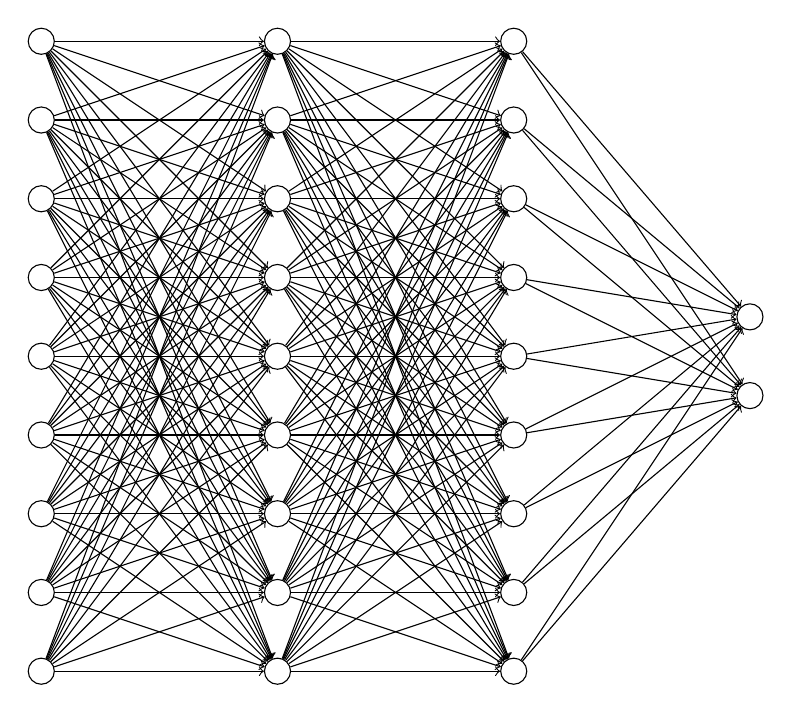
\begin{tikzpicture}[xscale = 3]
  \node[draw, circle] (N11) at (0, 0){
  };

  \node[draw, circle] (N21) at (0, -1){
  };

  \node[draw, circle] (N31) at (0, -2){
  };

  \node[draw, circle] (N41) at (0, -3){
  };

  \node[draw, circle] (N51) at (0, -4){
  };

  \node[draw, circle] (N61) at (0, -5){
  };

  \node[draw, circle] (N71) at (0, -6){
  };

  \node[draw, circle] (N81) at (0, -7){
  };

  \node[draw, circle] (N91) at (0, -8){
  };

  \node[draw, circle] (N12) at (1, 0){
  };

  \node[draw, circle] (N22) at (1, -1){
  };

  \node[draw, circle] (N32) at (1, -2){
  };

  \node[draw, circle] (N42) at (1, -3){
  };

  \node[draw, circle] (N52) at (1, -4){
  };

  \node[draw, circle] (N62) at (1, -5){
  };

  \node[draw, circle] (N72) at (1, -6){
  };

  \node[draw, circle] (N82) at (1, -7){
  };

  \node[draw, circle] (N92) at (1, -8){
  };

  \node[draw, circle] (N13) at (2, 0){
  };

  \node[draw, circle] (N23) at (2, -1){
  };

  \node[draw, circle] (N33) at (2, -2){
  };

  \node[draw, circle] (N43) at (2, -3){
  };

  \node[draw, circle] (N53) at (2, -4){
  };

  \node[draw, circle] (N63) at (2, -5){
  };

  \node[draw, circle] (N73) at (2, -6){
  };

  \node[draw, circle] (N83) at (2, -7){
  };

  \node[draw, circle] (N93) at (2, -8){
  };

  \node[draw, circle] (N14) at (3, -3.5){
  };

  \node[draw, circle] (N24) at (3, -4.5){
  };

  \draw[->] (N11) -- (N12);
  \draw[->] (N11) -- (N22);
  \draw[->] (N11) -- (N32);
  \draw[->] (N11) -- (N42);
  \draw[->] (N11) -- (N52);
  \draw[->] (N11) -- (N62);
  \draw[->] (N11) -- (N72);
  \draw[->] (N11) -- (N82);
  \draw[->] (N11) -- (N92);
  \draw[->] (N21) -- (N12);
  \draw[->] (N21) -- (N22);
  \draw[->] (N21) -- (N32);
  \draw[->] (N21) -- (N42);
  \draw[->] (N21) -- (N52);
  \draw[->] (N21) -- (N62);
  \draw[->] (N21) -- (N72);
  \draw[->] (N21) -- (N82);
  \draw[->] (N21) -- (N92);
  \draw[->] (N31) -- (N12);
  \draw[->] (N31) -- (N22);
  \draw[->] (N31) -- (N32);
  \draw[->] (N31) -- (N42);
  \draw[->] (N31) -- (N52);
  \draw[->] (N31) -- (N62);
  \draw[->] (N31) -- (N72);
  \draw[->] (N31) -- (N82);
  \draw[->] (N31) -- (N92);
  \draw[->] (N41) -- (N12);
  \draw[->] (N41) -- (N22);
  \draw[->] (N41) -- (N32);
  \draw[->] (N41) -- (N42);
  \draw[->] (N41) -- (N52);
  \draw[->] (N41) -- (N62);
  \draw[->] (N41) -- (N72);
  \draw[->] (N41) -- (N82);
  \draw[->] (N41) -- (N92);
  \draw[->] (N51) -- (N12);
  \draw[->] (N51) -- (N22);
  \draw[->] (N51) -- (N32);
  \draw[->] (N51) -- (N42);
  \draw[->] (N51) -- (N52);
  \draw[->] (N51) -- (N62);
  \draw[->] (N51) -- (N72);
  \draw[->] (N51) -- (N82);
  \draw[->] (N51) -- (N92);
  \draw[->] (N61) -- (N12);
  \draw[->] (N61) -- (N22);
  \draw[->] (N61) -- (N32);
  \draw[->] (N61) -- (N42);
  \draw[->] (N61) -- (N52);
  \draw[->] (N61) -- (N62);
  \draw[->] (N61) -- (N72);
  \draw[->] (N61) -- (N82);
  \draw[->] (N61) -- (N92);
  \draw[->] (N71) -- (N12);
  \draw[->] (N71) -- (N22);
  \draw[->] (N71) -- (N32);
  \draw[->] (N71) -- (N42);
  \draw[->] (N71) -- (N52);
  \draw[->] (N71) -- (N62);
  \draw[->] (N71) -- (N72);
  \draw[->] (N71) -- (N82);
  \draw[->] (N71) -- (N92);
  \draw[->] (N81) -- (N12);
  \draw[->] (N81) -- (N22);
  \draw[->] (N81) -- (N32);
  \draw[->] (N81) -- (N42);
  \draw[->] (N81) -- (N52);
  \draw[->] (N81) -- (N62);
  \draw[->] (N81) -- (N72);
  \draw[->] (N81) -- (N82);
  \draw[->] (N81) -- (N92);
  \draw[->] (N91) -- (N12);
  \draw[->] (N91) -- (N22);
  \draw[->] (N91) -- (N32);
  \draw[->] (N91) -- (N42);
  \draw[->] (N91) -- (N52);
  \draw[->] (N91) -- (N62);
  \draw[->] (N91) -- (N72);
  \draw[->] (N91) -- (N82);
  \draw[->] (N91) -- (N92);
  \draw[->] (N12) -- (N13);
  \draw[->] (N12) -- (N23);
  \draw[->] (N12) -- (N33);
  \draw[->] (N12) -- (N43);
  \draw[->] (N12) -- (N53);
  \draw[->] (N12) -- (N63);
  \draw[->] (N12) -- (N73);
  \draw[->] (N12) -- (N83);
  \draw[->] (N12) -- (N93);
  \draw[->] (N22) -- (N13);
  \draw[->] (N22) -- (N23);
  \draw[->] (N22) -- (N33);
  \draw[->] (N22) -- (N43);
  \draw[->] (N22) -- (N53);
  \draw[->] (N22) -- (N63);
  \draw[->] (N22) -- (N73);
  \draw[->] (N22) -- (N83);
  \draw[->] (N22) -- (N93);
  \draw[->] (N32) -- (N13);
  \draw[->] (N32) -- (N23);
  \draw[->] (N32) -- (N33);
  \draw[->] (N32) -- (N43);
  \draw[->] (N32) -- (N53);
  \draw[->] (N32) -- (N63);
  \draw[->] (N32) -- (N73);
  \draw[->] (N32) -- (N83);
  \draw[->] (N32) -- (N93);
  \draw[->] (N42) -- (N13);
  \draw[->] (N42) -- (N23);
  \draw[->] (N42) -- (N33);
  \draw[->] (N42) -- (N43);
  \draw[->] (N42) -- (N53);
  \draw[->] (N42) -- (N63);
  \draw[->] (N42) -- (N73);
  \draw[->] (N42) -- (N83);
  \draw[->] (N42) -- (N93);
  \draw[->] (N52) -- (N13);
  \draw[->] (N52) -- (N23);
  \draw[->] (N52) -- (N33);
  \draw[->] (N52) -- (N43);
  \draw[->] (N52) -- (N53);
  \draw[->] (N52) -- (N63);
  \draw[->] (N52) -- (N73);
  \draw[->] (N52) -- (N83);
  \draw[->] (N52) -- (N93);
  \draw[->] (N62) -- (N13);
  \draw[->] (N62) -- (N23);
  \draw[->] (N62) -- (N33);
  \draw[->] (N62) -- (N43);
  \draw[->] (N62) -- (N53);
  \draw[->] (N62) -- (N63);
  \draw[->] (N62) -- (N73);
  \draw[->] (N62) -- (N83);
  \draw[->] (N62) -- (N93);
  \draw[->] (N72) -- (N13);
  \draw[->] (N72) -- (N23);
  \draw[->] (N72) -- (N33);
  \draw[->] (N72) -- (N43);
  \draw[->] (N72) -- (N53);
  \draw[->] (N72) -- (N63);
  \draw[->] (N72) -- (N73);
  \draw[->] (N72) -- (N83);
  \draw[->] (N72) -- (N93);
  \draw[->] (N82) -- (N13);
  \draw[->] (N82) -- (N23);
  \draw[->] (N82) -- (N33);
  \draw[->] (N82) -- (N43);
  \draw[->] (N82) -- (N53);
  \draw[->] (N82) -- (N63);
  \draw[->] (N82) -- (N73);
  \draw[->] (N82) -- (N83);
  \draw[->] (N82) -- (N93);
  \draw[->] (N92) -- (N13);
  \draw[->] (N92) -- (N23);
  \draw[->] (N92) -- (N33);
  \draw[->] (N92) -- (N43);
  \draw[->] (N92) -- (N53);
  \draw[->] (N92) -- (N63);
  \draw[->] (N92) -- (N73);
  \draw[->] (N92) -- (N83);
  \draw[->] (N92) -- (N93);
  \draw[->] (N13) -- (N14);
  \draw[->] (N13) -- (N24);
  \draw[->] (N23) -- (N14);
  \draw[->] (N23) -- (N24);
  \draw[->] (N33) -- (N14);
  \draw[->] (N33) -- (N24);
  \draw[->] (N43) -- (N14);
  \draw[->] (N43) -- (N24);
  \draw[->] (N53) -- (N14);
  \draw[->] (N53) -- (N24);
  \draw[->] (N63) -- (N14);
  \draw[->] (N63) -- (N24);
  \draw[->] (N73) -- (N14);
  \draw[->] (N73) -- (N24);
  \draw[->] (N83) -- (N14);
  \draw[->] (N83) -- (N24);
  \draw[->] (N93) -- (N14);
  \draw[->] (N93) -- (N24);

\end{tikzpicture}

    }
  };

  \node (predTeacher) at (10, 2) {
    \scalebox{0.25}{
      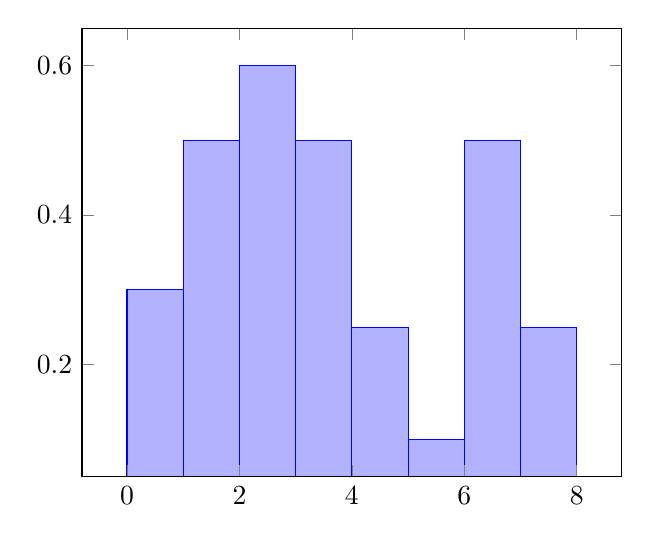
\begin{tikzpicture}
  \begin{axis}[
            area style,
            ]
    \addplot+[ybar interval,mark=no] plot coordinates {
      (0,.3)
      (1,.5)
      (2,.6)
      (3,.5)
      (4,.25)
      (5,.1)
      (6,.5)
      (7,.25)
      (8,.1)
    };
  \end{axis}
\end{tikzpicture}

    }
  };

  \node (predStudent) at (10, -2) {
    \scalebox{0.25}{
      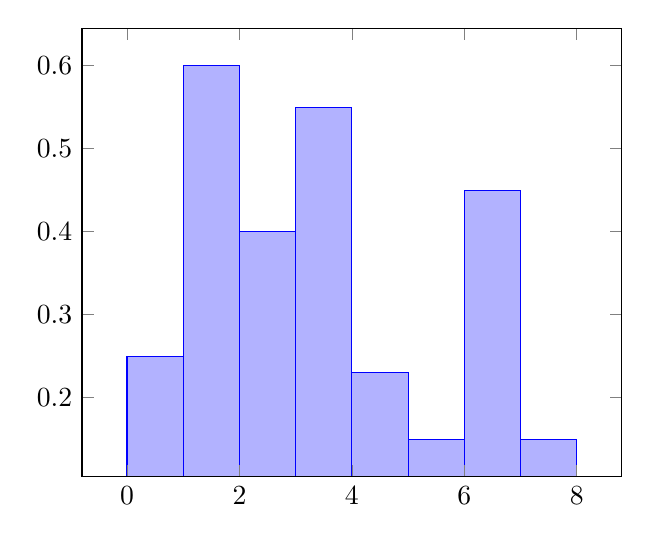
\begin{tikzpicture}
  \begin{axis}[
            area style,
            ]
    \addplot+[ybar interval,mark=no] plot coordinates {
      (0,.25)
      (1,.6)
      (2,.4)
      (3,.55)
      (4,.23)
      (5,.15)
      (6,.45)
      (7,.15)
      (8,.18)
    };
  \end{axis}
\end{tikzpicture}

    }
  };

  \draw[->, thick] (cleanImage) -- node [below = 0.05cm] {\rotatebox{-35}{\tiny pertubation}} (perturbedImage);
  \draw[->, thick] (cleanImage) -- (teacher);
  \draw[->, thick] (perturbedImage) -- (student);
  \draw[->, thick] (teacher) -- (predTeacher);
  \draw[->, thick] (student) -- (predStudent);
  \draw[<->, thick] (predTeacher) -- node [left = 0.3cm] {\small Consistency loss (MSE, KL div)} (predStudent);
\end{tikzpicture}
